\documentclass[tikz,border=5pt]{standalone}
\usepackage{luatexja}
\usepackage[hiragino-pron]{luatexja-preset}
\usepackage{amsmath,amssymb}
\usetikzlibrary{arrows.meta,patterns}

\begin{document}
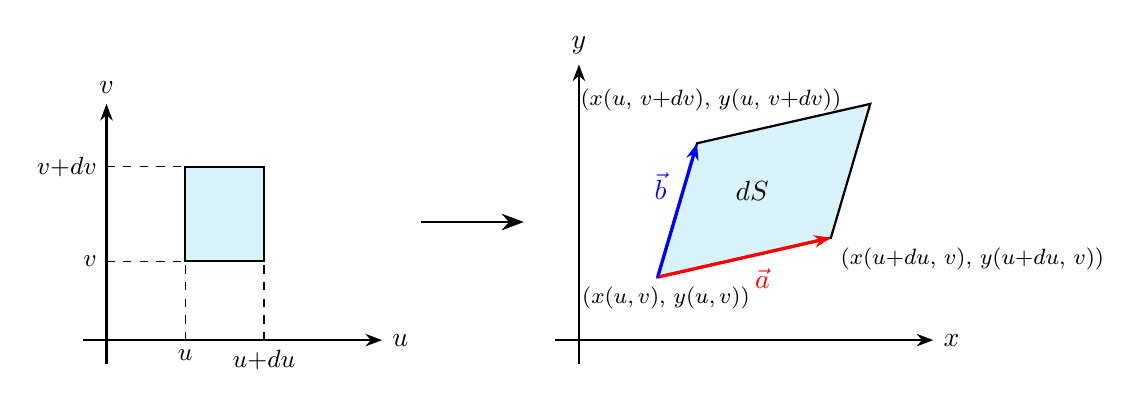
\begin{tikzpicture}[scale=1.0]

% uv-plane (left)
\begin{scope}[shift={(-4.5,0)}]
  \draw[-{Stealth[length=6pt]}, thick] (-0.3,0) -- (3.5,0) node[right] {$u$};
  \draw[-{Stealth[length=6pt]}, thick] (0,-0.3) -- (0,3) node[above] {$v$};

  % Rectangle
  \fill[cyan, opacity=0.15] (1,1) rectangle (2,2.2);
  \draw[thick] (1,1) rectangle (2,2.2);
  \draw[dashed, thin] (1,0) -- (1,1);
  \draw[dashed, thin] (2,0) -- (2,1);
  \draw[dashed, thin] (0,1) -- (1,1);
  \draw[dashed, thin] (0,2.2) -- (1,2.2);

  \node[below] at (1,0) {\small $u$};
  \node[below] at (2,0) {\small $u{+}du$};
  \node[left] at (0,1) {\small $v$};
  \node[left] at (0,2.2) {\small $v{+}dv$};
\end{scope}

% Arrow
\draw[-{Stealth[length=8pt]}, thick] (-0.5,1.5) -- (0.8,1.5);

% xy-plane (right)
\begin{scope}[shift={(1.5,0)}]
  \draw[-{Stealth[length=6pt]}, thick] (-0.3,0) -- (4.5,0) node[right] {$x$};
  \draw[-{Stealth[length=6pt]}, thick] (0,-0.3) -- (0,3.5) node[above] {$y$};

  % Parallelogram
  \coordinate (O) at (1,0.8);
  \coordinate (A) at (3.2,1.3);
  \coordinate (B) at (1.5,2.5);
  \coordinate (C) at (3.7,3.0);

  \fill[cyan, opacity=0.15] (O) -- (A) -- (C) -- (B) -- cycle;
  \draw[thick] (O) -- (A) -- (C) -- (B) -- cycle;

  % Vectors
  \draw[-{Stealth[length=6pt]}, very thick, red] (O) -- (A) node[midway, below right] {$\vec{a}$};
  \draw[-{Stealth[length=6pt]}, very thick, blue] (O) -- (B) node[midway, above left] {$\vec{b}$};

  % dS label
  \node at (2.2,1.9) {$dS$};

  % Point labels
  \node[below, font=\footnotesize, xshift=3pt] at (O) {$(x(u,v),\, y(u,v))$};
  \node[below right, font=\footnotesize] at (A) {$(x(u{+}du,\, v),\, y(u{+}du,\, v))$};
  \node[above, font=\footnotesize, xshift=5pt, yshift=8pt] at (B) {$(x(u,\, v{+}dv),\, y(u,\, v{+}dv))$};
\end{scope}

\end{tikzpicture}
\end{document}
